\documentclass{beamer}
\usepackage{tikz}
\usepackage{listings}

\usetheme{Singapore}
\usetikzlibrary{calc}

\title{Solitaire}


\makeatletter

\newcommand{\successors}{\mathrm{succ}}
\newcommand{\draw@stone}[1]{\shadedraw[ball color=gray,shading=ball] #1 circle (.25cm)}
\newcommand{\draw@hole}[1]{\draw[fill=gray!50] #1 circle (.125cm)}
\newcommand{\configuration}[2]{
  \foreach[count=\i] \x in {#1} {
    \csname draw@\x\endcsname{($ #2 + (\i * 0.75,0)$)};
  }
}

\makeatother


\begin{document}

\begin{frame}
  \titlepage
\end{frame}

\begin{frame}
  \frametitle{General Approach}
  \begin{enumerate}
    \item Start with initial configuration
    \item Perform all possible moves till we reach final configurations
    \item Keep only those that have one stone left
    \item Find the configuration with the leftmost stone
  \end{enumerate}
\end{frame}

\begin{frame}
  \frametitle{Visualized}
  \begin{itemize}
    \item Initial configuration
      \begin{center}
        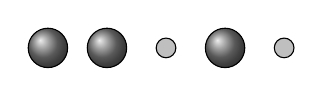
\begin{tikzpicture}
          \configuration{stone,stone,hole,stone,hole}{(2.5,0)}
        \end{tikzpicture}
      \end{center}
      \vskip5mm
    \item After one move
      \begin{center}
        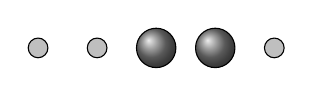
\begin{tikzpicture}
          \configuration{hole,hole,stone,stone,hole}{(0,1)}
        \end{tikzpicture}
      \end{center}
      \vskip5mm
    \item After two moves
      \begin{center}
        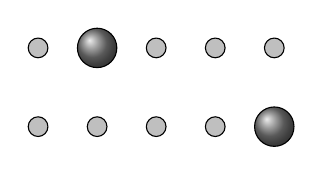
\begin{tikzpicture}
          \configuration{hole,stone,hole,hole,hole}{(0,0)}
          \configuration{hole,hole,hole,hole,stone}{(0,-1)}
        \end{tikzpicture}
      \end{center}
      \vskip5mm
    \item Winner:
      \begin{center}
        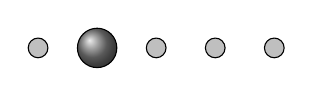
\begin{tikzpicture}
          \configuration{hole,stone,hole,hole,hole}{(0,0)}
        \end{tikzpicture}
      \end{center}
  \end{itemize}
\end{frame}

\begin{frame}
  \frametitle{Successors}
  \begin{itemize}
    \item Given an initial configuration $A$
      \begin{center}
        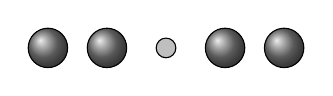
\begin{tikzpicture}
          \configuration{stone,stone,hole,stone,stone}{(0,0)}
        \end{tikzpicture}
      \end{center}
      \vskip5mm
    \item We can reach the following configurations $B_1, B_2$ using \emph{one} move
      \begin{center}
        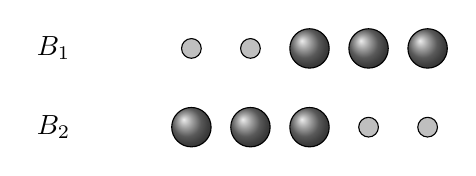
\begin{tikzpicture}
          \node at (-1,0) {$B_1$};
          \node at (-1,-1) {$B_2$};
          \configuration{hole,hole,stone,stone,stone}{(0,0)}
          \configuration{stone,stone,stone,hole,hole}{(0,-1)}
        \end{tikzpicture}
      \end{center}
      \vskip5mm
    \item These two configurations are \emph{successors} of the initial one
       \[
         \successors(A) = \{ B_1, B_2 \}
       \]
  \end{itemize}
\end{frame}

\begin{frame}
  \frametitle{Property of Successors}
  \begin{center} \bf
    A successor of configuration A has one stone less than~A
  \end{center}
  \vskip5mm
  \structure{Example}
  \begin{itemize}
    \item Original configuration
         \begin{center}
           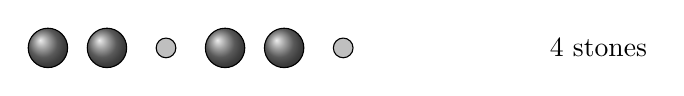
\begin{tikzpicture}
             \configuration{stone,stone,hole,stone,stone,hole}{(0,0)}
             \node[anchor=west] at (7,0) {4 stones};
           \end{tikzpicture}
         \end{center}
         \vskip5mm
    \item Successors
         \begin{center}
           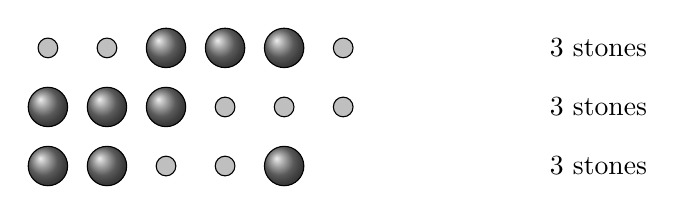
\begin{tikzpicture}
             \configuration{hole,hole,stone,stone,stone,hole}{(0,0)}
             \node[anchor=west] at (7,0) {3 stones};
             \configuration{stone,stone,stone,hole,hole,hole}{(0,-0.75)}
             \node[anchor=west] at (7,-0.75) {3 stones};
             \configuration{stone,stone,hole,hole,stone}{(0,-1.5)}
             \node[anchor=west] at (7,-1.5) {3 stones};
           \end{tikzpicture}
         \end{center}
  \end{itemize}
\end{frame}

\begin{frame}
  \frametitle{Using This Property}
  \begin{itemize}
    \item We are given an initial configuration, say with $N$ stones
    \item We want to find successors-of-successors-of-\dots with only 1 stone left
    \item $\Rightarrow$ We need to compute the $(N-1)$th successors
  \end{itemize}
  \begin{center}
    \begin{minipage}{.9\linewidth}
      \lstinputlisting[basicstyle=\small,flexiblecolumns=true]{guide-code.pseudo}
    \end{minipage}
  \end{center}
\end{frame}

\begin{frame}
  \frametitle{Step 1}
  \begin{center}
    \bf Find a way to recognize where jumps are possible
  \end{center}
  \begin{center}
    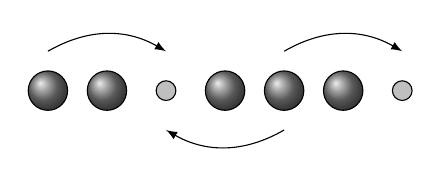
\begin{tikzpicture}
      \configuration{stone,stone,hole,stone,stone,stone,hole}{(0,0)}
      \draw[-latex] (0.75,0.5) to[bend left=30] ++(1.5,0);
      \draw[-latex] (3.75,0.5) to[bend left=30] ++(1.5,0);
      \draw[-latex] (3.75,-0.5) to[bend left=30] ++(-1.5,0);
    \end{tikzpicture}
  \end{center}
\end{frame}

\begin{frame}
  \frametitle{Step 2}
  \begin{center}
    \bf Find a way to compute the results of a jump
  \end{center}
  \begin{center}
    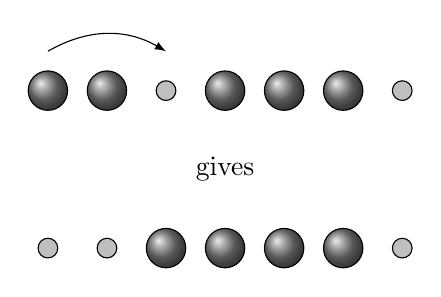
\begin{tikzpicture}
      \configuration{stone,stone,hole,stone,stone,stone,hole}{(0,0)}
      \draw[-latex] (0.75,0.5) to[bend left=30] ++(1.5,0);
      \node at (3,-1) {gives};
      \configuration{hole,hole,stone,stone,stone,stone,hole}{(0,-2)}
    \end{tikzpicture}
  \end{center}
\end{frame}

\begin{frame}
  \frametitle{Step 3}
  \begin{center}
    \bf Find a way to compute all successors of a given configuration
  \end{center}
  \begin{center}
    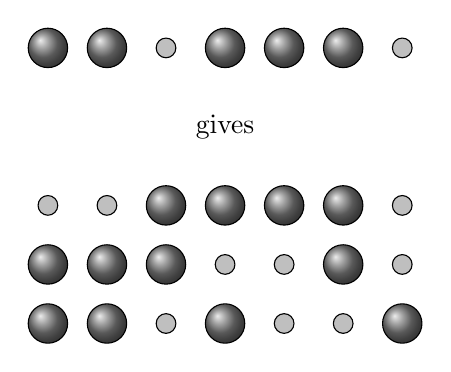
\begin{tikzpicture}
      \configuration{stone,stone,hole,stone,stone,stone,hole}{(0,0)}
      \node at (3,-1) {gives};
      \configuration{hole,hole,stone,stone,stone,stone,hole}{(0,-2)}
      \configuration{stone,stone,stone,hole,hole,stone,hole}{(0,-2.75)}
      \configuration{stone,stone,hole,stone,hole,hole,stone}{(0,-3.5)}
    \end{tikzpicture}
  \end{center}
\end{frame}

\begin{frame}
  \frametitle{Step 4}
  \begin{center}
    \bf Compute all successors of a set of configurations
  \end{center}
  \begin{center}
    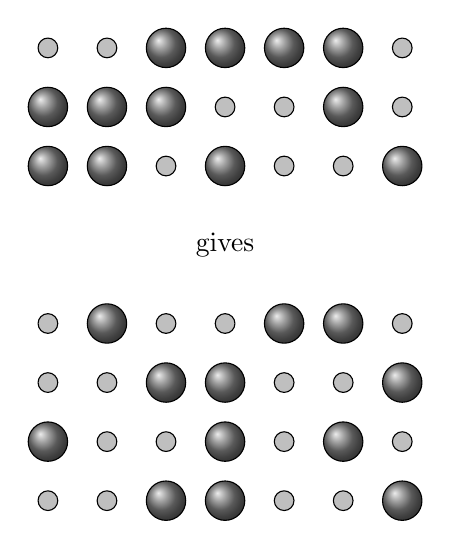
\begin{tikzpicture}
      \configuration{hole,hole,stone,stone,stone,stone,hole}{(0,0)}
      \configuration{stone,stone,stone,hole,hole,stone,hole}{(0,-.75)}
      \configuration{stone,stone,hole,stone,hole,hole,stone}{(0,-1.5)}
      \node at (3,-2.5) {gives};
      \configuration{hole,stone,hole,hole,stone,stone,hole}{(0,-3.5)}
      \configuration{hole,hole,stone,stone,hole,hole,stone}{(0,-4.25)}
      \configuration{stone,hole,hole,stone,hole,stone,hole}{(0,-5)}
      \configuration{hole,hole,stone,stone,hole,hole,stone}{(0,-5.75)}
    \end{tikzpicture}
  \end{center}
\end{frame}

\begin{frame}
  \frametitle{Step 5}
  \begin{center}
    \bf Do this to {\tt \{ initialConfiguration \}} $N-1$ times,
    where $N$ is the number of stones in {\tt initialConfiguration}
  \end{center}
\end{frame}

\end{document}